\documentclass[tikz,border=6pt]{standalone}
\usepackage[T1]{fontenc}
\usepackage{lmodern}
\usetikzlibrary{arrows.meta,positioning,fit,backgrounds,calc}
\definecolor{inA}{HTML}{DBE4FF}
\definecolor{ext}{HTML}{FFF3BF}
\definecolor{mdl}{HTML}{FFE8CC}
\definecolor{dec}{HTML}{E6FCF5}
\definecolor{out}{HTML}{D3F9D8}
\definecolor{ink}{HTML}{1F2933}
\hyphenpenalty=10000
\exhyphenpenalty=10000
\begin{document}
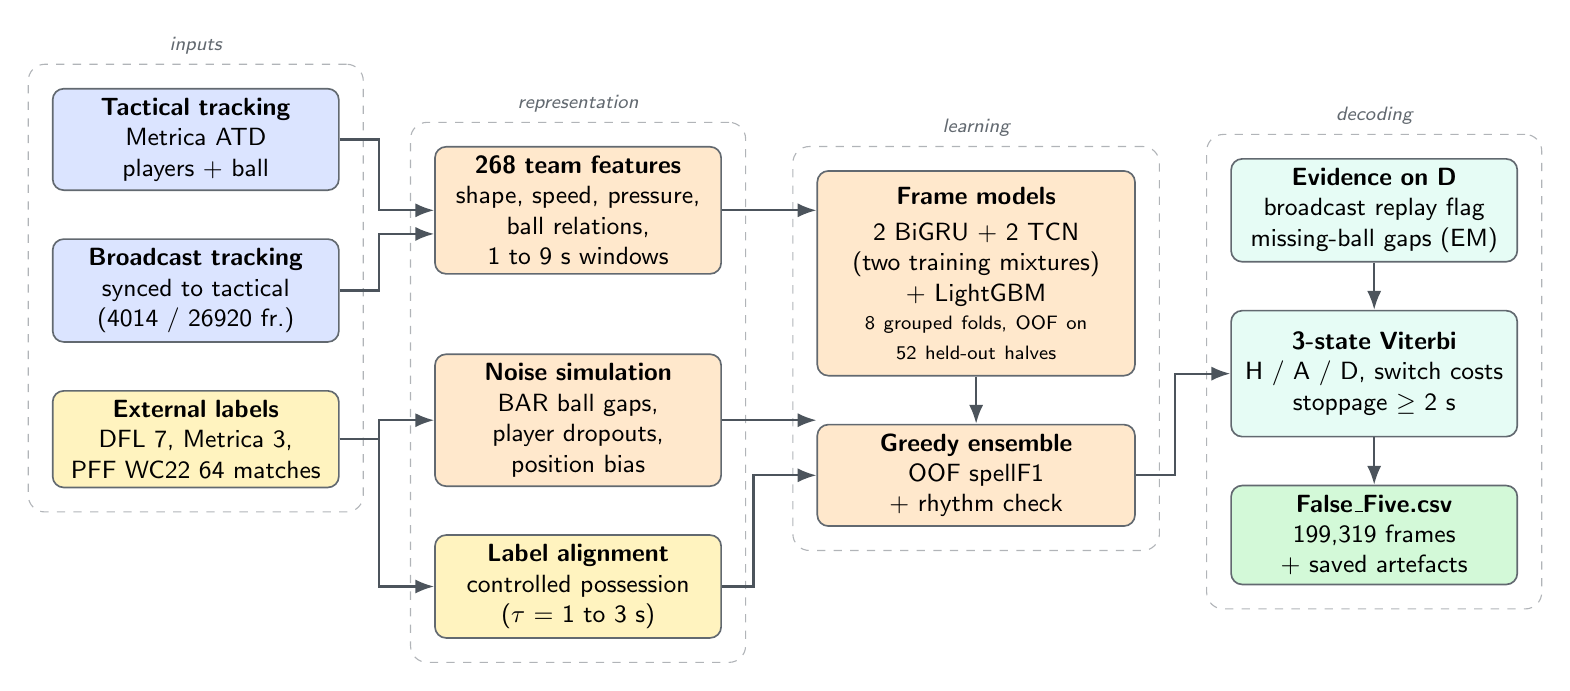
\begin{tikzpicture}[
  font=\sffamily\small, node distance=6mm and 7mm,
  box/.style={draw=ink!70, rounded corners=4pt, align=center, minimum height=12mm, text width=34mm, line width=0.6pt},
  arr/.style={-{Latex[length=2.4mm]}, line width=0.8pt, draw=ink!80},
  lab/.style={font=\sffamily\scriptsize\itshape, text=ink!70}]

% inputs
\node[box, fill=inA] (atd) {\textbf{Tactical tracking}\\Metrica ATD\\players + ball};
\node[box, fill=inA, below=of atd] (bro) {\textbf{Broadcast tracking}\\synced to tactical\\(4014 / 26920 fr.)};
\node[box, fill=ext, below=of bro] (extd) {\textbf{External labels}\\DFL 7, Metrica 3,\\PFF WC22 64 matches};

% representation
\node[box, fill=mdl, right=12mm of atd, yshift=-9mm] (feat) {\textbf{268 team features}\\shape, speed, pressure,\\ball relations,\\1 to 9 s windows};
\node[box, fill=mdl, below=10mm of feat] (sim) {\textbf{Noise simulation}\\BAR ball gaps,\\player dropouts,\\position bias};
\node[box, fill=ext, below=of sim] (align) {\textbf{Label alignment}\\controlled possession\\($\tau$ = 1 to 3 s)};

% learning
\node[box, fill=mdl, right=12mm of feat, text width=38mm, minimum height=26mm, yshift=-8mm] (models)
 {\textbf{Frame models}\\[2pt] 2 BiGRU + 2 TCN\\(two training mixtures)\\+ LightGBM\\[2pt]\scriptsize 8 grouped folds, OOF on\\52 held-out halves};
\node[box, fill=mdl, below=of models, text width=38mm] (ens) {\textbf{Greedy ensemble}\\OOF spellF1\\+ rhythm check};

% decoding
\node[box, fill=dec, right=12mm of models, yshift=8mm] (evid) {\textbf{Evidence on D}\\broadcast replay flag\\missing-ball gaps (EM)};
\node[box, fill=dec, below=of evid, minimum height=16mm] (vit) {\textbf{3-state Viterbi}\\H / A / D, switch costs\\stoppage $\geq$ 2 s};
\node[box, fill=out, below=of vit] (csv) {\textbf{False\_Five.csv}\\199,319 frames\\+ saved artefacts};

\draw[arr] (atd.east) -- ++(5mm,0) |- (feat.west);
\draw[arr] (bro.east) -- ++(5mm,0) |- ([yshift=-3mm]feat.west);
\draw[arr] (extd.east) -- ++(5mm,0) |- (sim.west);
\draw[arr] (extd.east) -- ++(5mm,0) |- (align.west);
\draw[arr] (feat.east) -- (feat.east -| models.west);
\draw[arr] (sim.east) -- (sim.east -| models.west);
\draw[arr] (align.east) -- ++(4mm,0) |- (ens.west);
\draw[arr] (models) -- (ens);
\draw[arr] (ens.east) -- ++(5mm,0) |- (vit.west);
\draw[arr] (evid) -- (vit);
\draw[arr] (vit) -- (csv);

\begin{scope}[on background layer]
\node[draw=ink!35, dashed, rounded corners=6pt, inner sep=3mm, fit=(atd)(bro)(extd), label={[lab]above:inputs}] {};
\node[draw=ink!35, dashed, rounded corners=6pt, inner sep=3mm, fit=(feat)(sim)(align), label={[lab]above:representation}] {};
\node[draw=ink!35, dashed, rounded corners=6pt, inner sep=3mm, fit=(models)(ens), label={[lab]above:learning}] {};
\node[draw=ink!35, dashed, rounded corners=6pt, inner sep=3mm, fit=(evid)(vit)(csv), label={[lab]above:decoding}] {};
\end{scope}
\end{tikzpicture}
\end{document}
